\documentclass[aspectratio=169,11pt]{beamer}
\usetheme{metropolis}
\metroset{block=fill, sectionpage=progressbar, numbering=fraction, progressbar=frametitle}

\usepackage{fontspec}
\setsansfont{Segoe UI}
\setmonofont{Consolas}
\usepackage{fvextra}
\usepackage{booktabs}
\usepackage{xcolor}

% ---- Palette (mềm, học thuật) — khớp deck tuần trước ----
\definecolor{deepteal}{HTML}{264653}
\definecolor{coral}{HTML}{E76F51}
\definecolor{tealc}{HTML}{2A9D8F}
\definecolor{cream}{HTML}{FBF9F5}
\definecolor{ink}{HTML}{233038}

\setbeamercolor{normal text}{fg=ink, bg=cream}
\setbeamercolor{frametitle}{fg=deepteal, bg=cream}
\setbeamercolor{title separator}{fg=coral}
\setbeamercolor{progress bar}{fg=coral}
\setbeamercolor{alerted text}{fg=coral}
\setbeamercolor{example text}{fg=tealc}
\setbeamercolor{itemize item}{fg=coral}
\setbeamercolor{itemize subitem}{fg=tealc}
\setbeamercolor{block title}{bg=tealc!18, fg=deepteal}
\setbeamercolor{block body}{bg=tealc!7}
\setbeamercolor{block title alerted}{bg=coral!20, fg=coral!60!black}
\setbeamercolor{block body alerted}{bg=coral!8}
\setbeamercolor{block title example}{bg=deepteal!12, fg=deepteal}
\setbeamercolor{block body example}{bg=deepteal!5}

\newcommand{\promptbox}[2]{\VerbatimInput[breaklines=true,breakanywhere=true,%
  breaksymbolleft={},breakautoindent=true,%
  fontsize=#1,baselinestretch=0.92,frame=single,framesep=4pt,%
  rulecolor=\color{deepteal!35},formatcom=\color{ink}]{#2}}
\newcommand{\take}[1]{\vfill{\footnotesize\color{deepteal}#1}}

\title{Tác nhân LLM trong trò chơi rủi ro tập thể — Tuần 2}
\subtitle{Hai mở rộng: \emph{phóng to model} (scaling) \& \emph{kiểm tra đọc-hiểu} (comprehension)}
\date{\today}
\author{Báo cáo nghiên cứu}

\begin{document}
\maketitle

% ======================================================================
\section{Tuần này làm gì}

\begin{frame}{Nhắc lại kết luận tuần trước (3 model nhỏ, baseline)}
  \begin{block}{LLM chơi collective-risk game KHÁC con người}
    \begin{itemize}
      \item \textbf{Phớt lờ rủi ro}: đạt mục tiêu $\sim$100\% ở cả 3 mức rủi ro (người: 50/10/0\%).
      \item \textbf{Hợp tác TĂNG dần} qua vòng, không phản bội cuối game (ngược người).
      \item \textbf{Vượt mục tiêu}: Qwen-7B $\sim$233, Llama-8B $\sim$185, Gemma-9B $\sim$129.
    \end{itemize}
  \end{block}
  \begin{exampleblock}{Hai câu hỏi còn treo $\Rightarrow$ hai thí nghiệm tuần này}
    \begin{enumerate}
      \item Các bất thường này có phải vì model \emph{nhỏ}? $\to$ \alert{Large model (scaling)}.
      \item Phớt-lờ-rủi-ro là \emph{không hiểu luật} hay \emph{cố tình}? $\to$ \alert{Comprehension}.
    \end{enumerate}
  \end{exampleblock}
\end{frame}

\begin{frame}{Thiết lập hai thí nghiệm mới}
  \begin{center}\small
  \begin{tabular}{lll}
    \toprule
    & \textbf{5 · Large model (scaling)} & \textbf{6 · Comprehension} \\
    \midrule
    Mục tiêu   & bất thường có do cỡ model? & model có HIỂU luật không? \\
    Model      & Qwen 7B$\to$32B, Gemma 9B$\to$27B & 3 model nhỏ (như baseline) \\
    Điều kiện  & baseline trung tính (y hệt tuần 1) & probe IN-SITU trong ván baseline \\
    Đo gì      & reach, đóng góp, vân tay, vòng & accuracy 20 câu hỏi/3 trục \\
    Quy mô     & 60 ván/model (3 risk×2 lang×10) & \,$\sim$54.5k probe/model \\
    \bottomrule
  \end{tabular}
  \end{center}
  \vfill
  \begin{block}{Comprehension — phỏng theo ``Nicer Than Humans'' (Fontana et al.\ 2024)}
    {\footnotesize Mỗi vòng bắn THÊM câu hỏi Rules / Time / State, gửi RIÊNG (không đụng quyết định), chấm so ground-truth của engine. Hai nhánh A/B: \texttt{showCumulative} pool ẩn (như baseline) vs pool hiện (tái lập Figure A7).}
  \end{block}
\end{frame}

% ======================================================================
\section{5 · Large model (scaling)}

\begin{frame}{Scaling — câu hỏi \& cách đọc}
  \begin{block}{Thao tác}
    {\footnotesize Giữ NGUYÊN prompt baseline trung tính của tuần 1, chỉ \textbf{thay model}: Qwen2.5-7B$\to$32B, Gemma-2-9B$\to$27B. Llama-3.1-8B giữ làm mốc tham chiếu. Cùng 3 mức rủi ro $\times$ \{EN, VN\} $\times$ 10 lần lặp.}
  \end{block}
  \begin{exampleblock}{Hai giả thuyết cạnh tranh}
    \begin{itemize}
      \item \emph{H1 — ``do model nhỏ''}: model lớn sẽ nhạy rủi ro hơn, giống người hơn.
      \item \emph{H2 — ``đặc tính bền''}: bất thường vẫn còn; chỉ phần \emph{kinh tế} thay đổi.
    \end{itemize}
  \end{exampleblock}
\end{frame}

\begin{frame}{Scaling — Qwen thôi hào phóng, hội tụ về ``vừa đủ 120''}
  \centering
\includegraphics[height=0.66\textheight]{figs/L1_scaling_contrib.png}
  \take{Phóng to Qwen 7B$\to$32B kéo đóng góp \alert{233$\to$128} ($-105$); Gemma 9B$\to$27B gần như đứng yên (129$\to$126). Model lớn hội tụ về cùng một chiến lược ``ép sát mục tiêu'' — Gemma vốn đã ở đó.}
\end{frame}

\begin{frame}{Scaling — KHÔNG phục hồi nhạy-rủi-ro (H2 thắng)}
  \centering
\includegraphics[height=0.66\textheight]{figs/L2_scaling_reach.png}
  \take{Cả Qwen-32B lẫn Gemma-27B vẫn đạt mục tiêu $\sim$100\% ở mọi mức rủi ro (đường người dốc 50$\to$10$\to$0\%). Phớt-lờ-rủi-ro \alert{bền theo cỡ model} — không phải lỗi của model nhỏ.}
\end{frame}

\begin{frame}{Scaling — ``vân tay'' lựa chọn LẬT về mức 2}
  \centering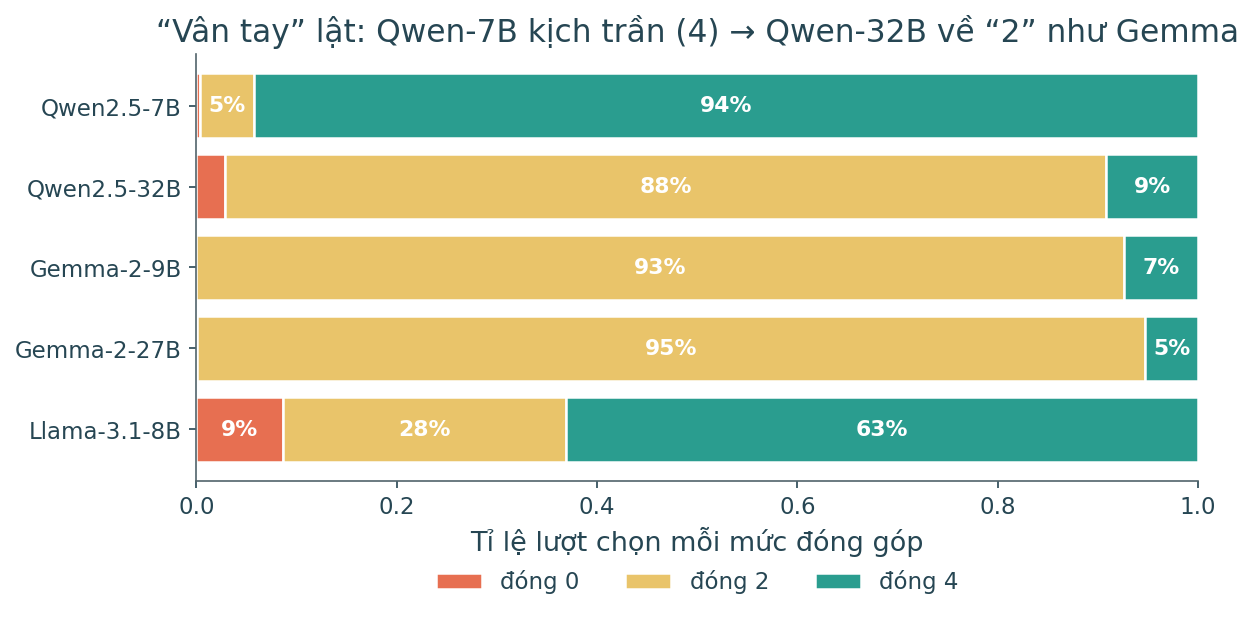
\includegraphics[height=0.64\textheight]{figs/L3_choice_flip.png}
  \take{Qwen-7B kịch trần (94\% chọn 4) nhưng Qwen-32B đổi sang \alert{88\% chọn 2} — đúng mức ``fair-share'' mà Gemma đã khoá. Model càng lớn càng kinh tế: bỏ thói quá-đóng-góp, chỉ đóng vừa đủ phần công bằng.}
\end{frame}

\begin{frame}{Scaling — vẫn tăng dần, ``ép vạch'' sát deadline}
  \centering
\includegraphics[height=0.64\textheight]{figs/L4_scaling_dynamics.png}
  \take{Model lớn giữ phẳng ở 2.0 gần hết game rồi \emph{ramp} ở vòng 9--10 (Gemma-27B: 2.0$\to$2.87). Vẫn là quỹ đạo \alert{tăng dần} ngược người — chỉ ``ép sát ngưỡng'' muộn và gọn hơn, tiết kiệm hơn model nhỏ.}
\end{frame}

\begin{frame}{Scaling — trục ngôn ngữ co lại (Llama vẫn lệch nhất)}
  \centering
\includegraphics[height=0.62\textheight]{figs/L5_scaling_lang.png}
  \take{Khoảng cách EN--VN của Qwen co từ $-10$ (7B) còn $-3$ (32B); Gemma-27B đảo dấu nhẹ ($-13$). Llama-8B vẫn lệch mạnh nhất ($-44$). Phóng to làm hành vi \emph{ổn định hơn} giữa hai ngôn ngữ, nhưng không xoá trục này.}
\end{frame}

\begin{frame}{Scaling — chốt phần 5}
  \begin{center}\small
  \begin{tabular}{lll}
    \toprule
    Khía cạnh & Nhỏ (7--9B) & Lớn (27--32B) \\
    \midrule
    Nhạy rủi ro          & Không (100\% phẳng) & \alert{Không} (100\% phẳng) \\
    Hợp tác qua vòng     & Tăng dần & \alert{Tăng dần} (ramp muộn) \\
    Mức đóng góp Qwen    & 233 (kịch trần 4) & \alert{128} (về mức 2) \\
    Mức đóng góp Gemma   & 129 & 126 (gần như không đổi) \\
    Tiền mặt giữ (Qwen)  & 7/240 & \alert{112/240} \\
    \bottomrule
  \end{tabular}
  \end{center}
  \take{Phóng to model = \emph{kinh tế hơn}, KHÔNG phải \emph{nhạy rủi ro hơn}. Bất thường cốt lõi (phớt-lờ-rủi-ro, tăng dần) là đặc tính bền, không phải hạn chế dung lượng.}
\end{frame}

% ======================================================================
\section{6 · Comprehension (đọc-hiểu)}

\begin{frame}[fragile]{Comprehension — thiết kế probe}
  \begin{block}{20 câu hỏi · 3 trục (chấm so ground-truth engine)}
    {\footnotesize \textbf{RULES} (luật tĩnh: mức đóng, vốn, mục tiêu, số vòng, \% rủi ro, payoff) ·
    \textbf{TIME} (tra lịch sử: đang vòng mấy, ai đóng bao nhiêu ở vòng $i$) ·
    \textbf{STATE} (thống kê tích luỹ: quỹ hiện có, còn thiếu bao nhiêu — phần lớn phải \emph{tự cộng dồn}).}
  \end{block}
  \promptbox{\fontsize{7.4}{8.6}\selectfont}{assets/probe_examples.txt}
  \take{Cùng một câu STATE: pool ẨN model đáp 24 (chỉ một vòng) thay vì 96; pool HIỆN đáp đúng ngay.}
\end{frame}

\begin{frame}{Comprehension — hiểu LUẬT \& đọc LỊCH SỬ tốt, sụp ở CỘNG DỒN}
  \centering
\includegraphics[height=0.64\textheight]{figs/K1_comp_category.png}
  \take{Rules 94--100\%, Time 82--99\% — model \emph{hiểu luật} và \emph{tra được lịch sử}. Nhưng State (cộng dồn) chỉ 32--72\%: Gemma 72\% $>$ Qwen 37\% $>$ Llama 32\%. Lỗ hổng nằm ở \alert{số học tích luỹ}, không phải ở luật chơi.}
\end{frame}

\begin{frame}{Comprehension — ĐỌC được $\neq$ CỘNG được (kết quả sắc nhất)}
  \centering
\includegraphics[height=0.62\textheight]{figs/K2_comp_read_vs_add.png}
  \take{Số IN SẴN trong prompt (own\_remaining): 66--100\%. Cùng loại ``tổng quỹ'' nhưng PHẢI cộng dồn: pool ẨN chỉ \alert{10--21\%}; khi prompt IN sẵn tổng thì vọt lên \alert{92--100\%}. Model \emph{đọc được nhưng không cộng được} — đúng Figure A7 của ``Nicer Than Humans''.}
\end{frame}

\begin{frame}{Comprehension — CỔNG: họ BIẾT rủi ro, chỉ là phớt lờ}
  \centering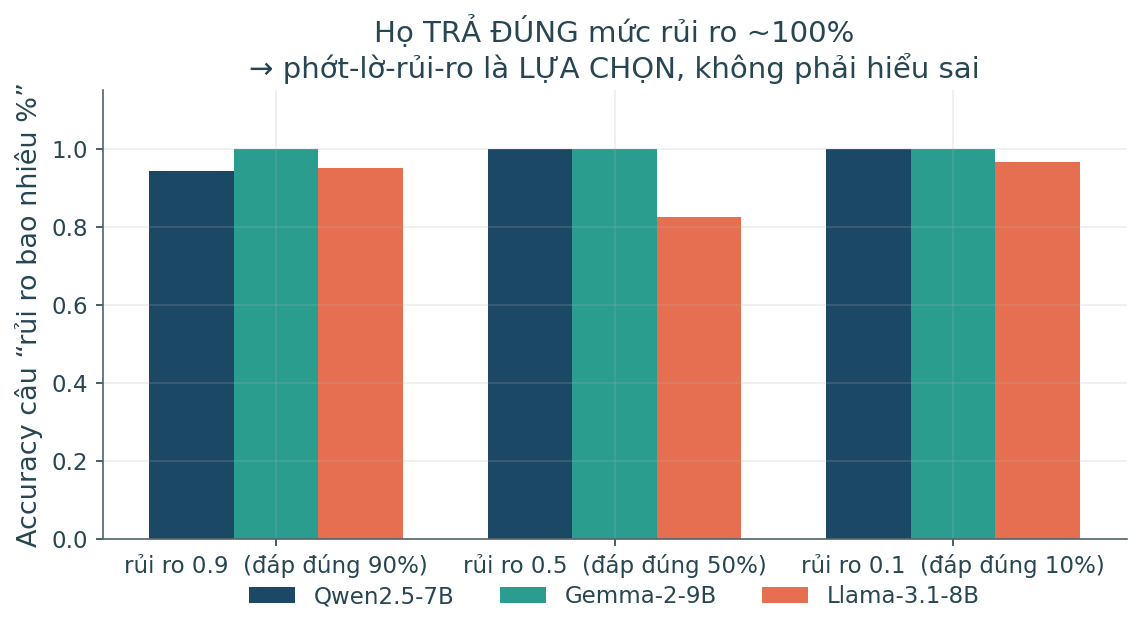
\includegraphics[height=0.60\textheight]{figs/K3_comp_risk_gate.png}
  \take{Câu ``rủi ro bao nhiêu \%'' được trả đúng $\sim$100\% (Qwen 98, Gemma 100, Llama 91). Vậy phớt-lờ-rủi-ro \alert{KHÔNG phải do hiểu sai luật} — model biết rõ 90/50/10\% nhưng vẫn chọn như nhau. Đây là \emph{cổng} hợp thức hoá claim hành vi của tuần trước.}
\end{frame}

\begin{frame}{Comprehension — tiếng Việt đánh đúng vào cộng dồn}
  \centering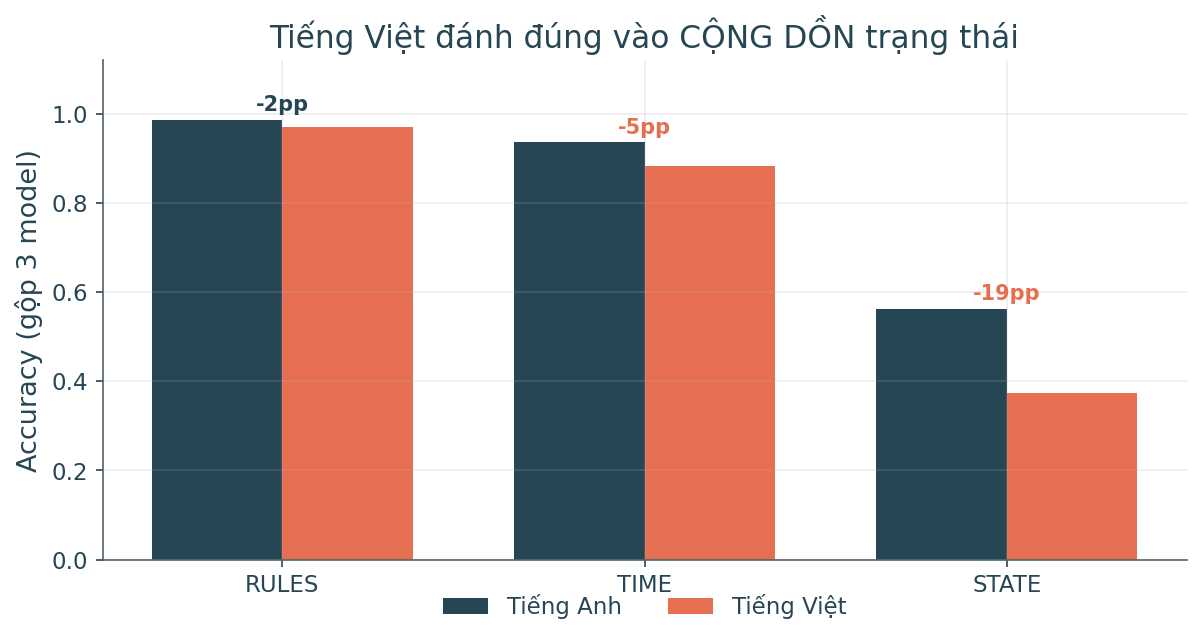
\includegraphics[height=0.60\textheight]{figs/K4_comp_lang.png}
  \take{Rules/Time gần như không đổi giữa EN/VN ($-2$/$-5$pp); nhưng State rớt \alert{$-19$pp} ở tiếng Việt (Gemma nặng nhất: $-32$pp). Trục ngôn ngữ tấn công đúng khâu yếu nhất — \emph{số học trạng thái} — chứ không phải khả năng đọc luật.}
\end{frame}

\begin{frame}{Comprehension — bảng chi tiết 20 câu (phụ lục)}
  \centering
\includegraphics[height=0.66\textheight]{figs/K5_comp_figure1.png}
  \take{Trần ở Rules; Time tốt trừ \texttt{time\_round\_total\_i} (phải cộng 6 ghế trong 1 vòng). State lủng đều: \texttt{state\_X\_total}, \texttt{state\_own\_total}, \texttt{state\_rounds\_left} đều thấp. Riêng \texttt{state\_pool} nhảy rõ giữa hai panel (ẩn$\to$hiện).}
\end{frame}

% ======================================================================
\section{Tổng hợp tuần 2}

\begin{frame}{Hai mảnh ghép vào bức tranh chung}
  \begin{block}{Cơ chế hợp tác của LLM = \emph{prior}, không phải \emph{tính toán}}
    \begin{itemize}
      \item \textbf{Comprehension}: model HIỂU luật \& BIẾT rủi ro (Rules $\sim$100\%, risk-gate $\sim$100\%) nhưng KHÔNG cộng được trạng thái (State 10--21\% khi phải tự tính).
      \item \textbf{Hệ quả}: hợp tác vẫn đạt mục tiêu \emph{dù} ghi sổ sai $\Rightarrow$ là thiên kiến hợp tác có sẵn, không phải suy luận chiến lược theo trạng thái.
      \item \textbf{Scaling}: phóng to chỉ cắt phần \emph{lãng phí} (Qwen 233$\to$128) — làm model \emph{kinh tế hơn}, nhưng giữ nguyên phớt-lờ-rủi-ro \& tăng-dần.
    \end{itemize}
  \end{block}
  \take{Phớt-lờ-rủi-ro KHÔNG phải lỗi hiểu (comprehension bác bỏ) cũng KHÔNG phải lỗi dung lượng (scaling bác bỏ) $\Rightarrow$ là một \alert{thiên kiến hành vi} của lớp model này.}
\end{frame}

\begin{frame}{So với tuần trước: cập nhật bảng tổng}
  \centering\small
  \begin{tabular}{lll}
    \toprule
    Câu hỏi & Trả lời tuần trước & Bằng chứng tuần này \\
    \midrule
    Do model nhỏ?            & (giả thuyết) & \alert{Không} — 27/32B vẫn phẳng 100\% \\
    Có hiểu luật không?      & (chưa đo)    & \alert{Có} — Rules 94--100\% \\
    Có biết mức rủi ro?      & (chưa đo)    & \alert{Có} — risk-gate $\sim$100\% \\
    Vì sao ghi sổ sai?       & ``hợp tác là prior'' & \alert{Không cộng dồn được} (State 10--21\%) \\
    Trục ngôn ngữ ở đâu?     & đóng góp (Llama) & + \alert{số học trạng thái} (State $-19$pp VN) \\
    \bottomrule
  \end{tabular}
  \take{Hai thí nghiệm \emph{khẳng định} và \emph{giải thích} các bất thường của tuần 1, thay vì lật chúng.}
\end{frame}

\begin{frame}{Điểm thảo luận với thầy}
  \textbf{Về scaling}
  \begin{itemize}
    \item Chưa có Llama lớn (70B) — có cần để hoàn tất cặp họ thứ ba?
    \item Qwen-32B tụt nhẹ reach (97\%) vì chơi sát vạch 120 — có nên báo cáo đóng góp làm biến chính (như đã chốt tuần trước)?
  \end{itemize}
  \textbf{Về comprehension}
  \begin{itemize}
    \item ``Không cộng dồn được'' là giới hạn số học hay do prompt quá dài? $\to$ đề xuất ablation \emph{độ dài lịch sử} (probe theo vòng).
    \item Có nên đưa \emph{một câu state-pool} vào prompt quyết định để xem hợp tác có đổi khi model ``được nhắc'' tổng quỹ?
  \end{itemize}
\end{frame}

\begin{frame}[standout]
  Phóng to model làm nó \textbf{kinh tế hơn}, không \textbf{nhạy rủi ro hơn}. \\[2mm]
  LLM \textbf{hiểu luật} và \textbf{biết rủi ro} — nhưng \textbf{không cộng được trạng thái}: \\
  hợp tác là \textbf{thiên kiến có sẵn}, không phải tính toán.
\end{frame}

\end{document}
